

\chapter{Potentials V(x,y,z)}

In this chapter we will find the intensity and the $\psi$ function of a particle under a potential. 

\section{Potential in 3 dimensions}

First, we need to define our energy and our equations in 3D, this equations can be obtained from the second chapter generalizing to 3 dimensions.

\begin{equation}
    \label{3.1}
    \frac{p_x^2+p_y^2+p_z^2}{2m}+V(x,y,z) = E
\end{equation}

\begin{equation}
    \label{3.2}
    \left[ -\frac{\hbar^2}{2m} \left[\frac{\partial^2}{\partial x^2}+\frac{\partial^2}{\partial y^2}+\frac{\partial^2}{\partial z^2}  \right] +V(x,y,z) \right] \psi = i\hbar \frac{\partial}{\partial t}\psi
\end{equation}

Where $\psi$ is a function of space and time, i.e. $\psi = \psi(x,y,z,t)$. Before doing some operations with this equations we want to define a boundary for the intensity function. When we talk about this function in the second chapter we define a boundary in \ref{int_P(x)_def}, we need to do the same but in 3 dimensions. 

\begin{equation}
    \label{3.3}
    \int_{-\infty}^{\infty}\int_{-\infty}^{\infty}\int_{-\infty}^{\infty}P(x,y,z)dxdydz = 1
\end{equation}

For this equation to be satisfied we need to achieve this properties:

\begin{itemize}
    \item $\lim_{x\to\infty}P(x,y,z) = 0$ $\forall y,z$
    \item $\lim_{y\to\infty}P(x,y,z) = 0$ $\forall x,z$ 
    \item $\lim_{z\to\infty}P(x,y,z) = 0$ $\forall x,y$ 
\end{itemize}

The intensity is define as $P(x,y,z,t) = \psi\psi^{\star}$. We have defined the intensity and we can continue now with Equation \ref{3.2}. To resolve this we will use the equation and it's conjugate and we will multiply for $\psi$ or $\psi^{\star}$. 

\begin{equation}
    \label{3.4}
    \begin{split}
        &\psi^{\star}\left[ -\frac{\hbar^2}{2m} \left[\frac{\partial^2}{\partial x^2}+\frac{\partial^2}{\partial y^2}+\frac{\partial^2}{\partial z^2}  \right] +V\right] \psi = i \psi^{\star}\hbar \frac{\partial}{\partial t}\psi
        \\
        &\psi\left[ -\frac{\hbar^2}{2m} \left[\frac{\partial^2}{\partial x^2}+\frac{\partial^2}{\partial y^2}+\frac{\partial^2}{\partial z^2}  \right] +V\right] \psi^{\star} = -i \psi \hbar \frac{\partial}{\partial t}\psi^{\star}
    \end{split}
\end{equation}

To continue we will subtract the first equation with the second one.

\begin{equation}
    \label{3.5}
    \begin{split}
        &\frac{\hbar^2}{2m}\left[ \psi \left[ \frac{\partial^2}{\partial x^2}+\frac{\partial^2}{\partial y^2}+\frac{\partial^2}{\partial z^2}\right]\psi^{\star} -\psi^{\star}\left[ \frac{\partial^2}{\partial x^2}+\frac{\partial^2}{\partial y^2}+\frac{\partial^2}{\partial z^2}\right]\psi\right] = i\hbar\left[\psi\frac{\partial}{\partial t}\psi^{\star}+\psi^{\star}\frac{\partial}{\partial t}\psi \right]
        \\
        &\frac{\hbar^2}{2m}\left[\frac{\partial}{\partial x}\left(\psi\frac{\partial}{\partial x}\psi^{\star}-\psi^{\star}\frac{\partial}{\partial x}\psi \right)+\frac{\partial}{\partial y}\left(\psi\frac{\partial}{\partial y}\psi^{\star}-\psi^{\star}\frac{\partial}{\partial y}\psi \right)+
        \\
        &+\frac{\partial}{\partial z}\left(\psi\frac{\partial}{\partial z}\psi^{\star}-\psi^{\star}\frac{\partial}{\partial z}\psi \right) \right] = i\hbar\left[\psi\frac{\partial}{\partial t}\psi^{\star}+\psi^{\star}\frac{\partial}{\partial t}\psi \right]
    \end{split}
\end{equation}

If we integrate both sides we get that the left side is 0.

\begin{equation}
    \label{3.6}
    \begin{split}
    &i\hbar \int_{-\infty}^{\infty}dx\int_{-\infty}^{\infty}dy\int_{-\infty}^{\infty}dz \left[\psi\frac{\partial}{\partial t}\psi^{\star}+\psi^{\star}\frac{\partial}{\partial t}\psi \right] = 0
    \\
    &\frac{d}{dt}\int_{-\infty}^{\infty}dx\int_{-\infty}^{\infty}dy\int_{-\infty}^{\infty}dz \psi \psi^{\star} = 0
    \end{split}
\end{equation}

This equation tell us that the total intensity must be constant among the time, so now we know the conditions of the intensity for space from \ref{3.3} and for time.

\section{Discontinuous Functions}

We will work in one dimension only for now on to get things easier. Some potentials are discontinuous function, one of the most common example is the square well potential. We want to study this discontinuous functions and for that we will recover the delta function.

\begin{marginfigure}
    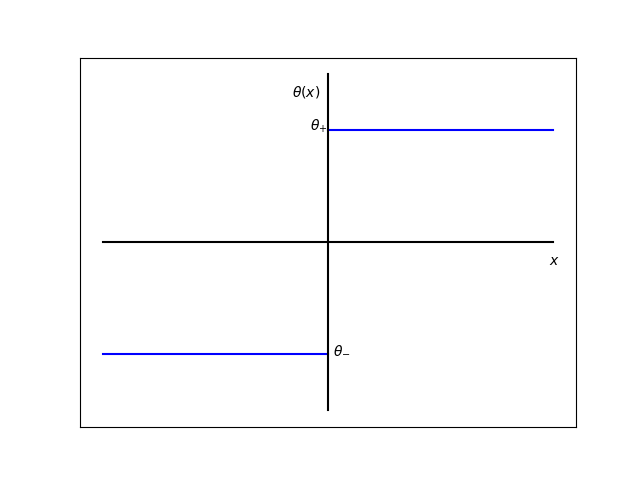
\includegraphics{images3/theta_func.png}
    \caption{Discontinuous function with a finite jump in x = 0}
    \label{theta_func}
\end{marginfigure}


We want to prove that: 

\begin{equation}
    \label{3.7}
    \frac{d\theta}{dx} = C \delta(x)
\end{equation}

This equation is true if: 

\begin{equation}
    \label{3.8}
    \int_{-\infty}^{\infty}f(x) \frac{d\theta}{dx} dx = f(0) C
\end{equation}

Because of the definition of the delta function. To prove this and also to get the value of C we need to operate carefully this integral.

\begin{equation}
    \label{3.9}
    \begin{split}
        &\int_{-\infty}^{\infty}\left( \frac{d}{dx}[f(x)\theta(x)]-\theta(x)\frac{df}{dx}\right)dx = 
        \\
        & = \left[ f(x) \theta(x) \right]_{-\infty}^{\infty}-\int_{-\infty}^{\infty}\frac{d\theta}{dx}\theta(x)dx =
        \\
        & = f(\infty)\theta_+ + f(-\infty)\theta_- + \theta_- \int_{-\infty}^{0}\frac{df}{dx}dx - \theta_+ \int_{0}^{\infty}\frac{df}{dx}dx = 
        \\
        & = f(\infty)\theta_+ + f(-\infty)\theta_- + \theta_- (f(0)-f(-\infty)) - \theta_+ (f(\infty)-f(0))=
        \\
        & = f(0) [\theta_- + \theta_+]
    \end{split}
\end{equation}

We prove that \ref{3.7} is true and also that C is the "jump" distance in the discontinuous function.

%%%%%% CONTINUE THIS PART LATER I DONT UNDERSTAND %%%%%%%%%%%


\section{Square Potential Well}

\begin{figure}[H]
    \centering
    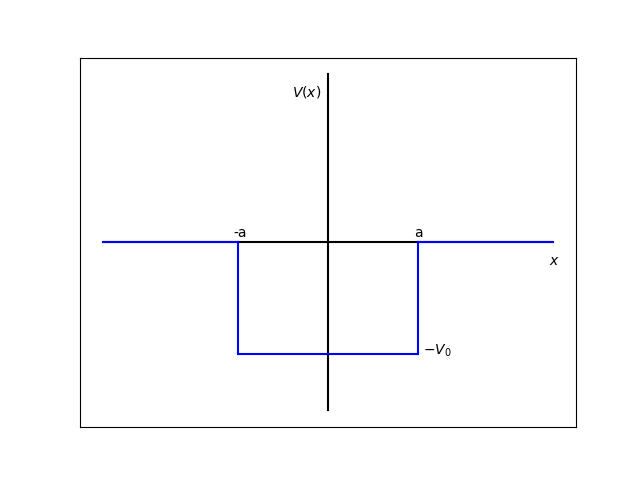
\includegraphics{images3/square_potential.png}
    \caption{Square Potential Well }
    \labfig{fig:square_potential}
\end{figure}

We have a potential as the one in \reffig{fig:square_potential} and we want to study the intensity and the $\psi$ function of a particle among space and time. First i have to define the potential.


\begin{equation}
    f(x) = \frac{-dV}{dx}
\end{equation}

In particle mechanics the problem will be solved with the equation of the energy.

\begin{equation}
    \label{3.11}
    E = \frac{1}{2}m\left(\frac{dx}{dt}\right)^2 + V(x) = constant
\end{equation}

In wave mechanics is more complex we will get the Schrödinguer Wave Equation for one dimension.

\begin{equation}
    \label{3.12}
    i\hbar \frac{\partial\psi(x,t)}{\partial t} = \frac{-\hbar^2}{2m}\frac{\partial^2\psi(x,t)}{\partial x^2} + V(x)\psi(x,t)
\end{equation}

Let's consider one solution to this equation.

\begin{equation}
    \label{3.13}
    \psi(x,t) = \phi(x)e^{-i\frac{E}{\hbar}t}
\end{equation}

Where $\phi(x)$ is a real function, if we remember we solved $\phi(x)$ for the free particle problem and it was a exponential.

\begin{equation}
    \label{3.14}
    \phi(x) = e^{ikx}
\end{equation}

This function does not fulfill equation \ref{3.3}.

\begin{equation}
    \label{3.15}
    \int_{-\infty}^{\infty} \phi^{\star}(x)\phi(x) dx = \infty
\end{equation}

This means that we only have solutions if $V(x) \neq 0$. 

Using our knowledge on the previous section we can get an expression for f(x).

\begin{equation}
    \label{3.16}
    f(x) = \frac{-dV}{dx} = - [ (-V_0-0)\delta(-a) + (0-(-V_0))\delta(a) ] = V_0\delta(-a)-V_0\delta(a)
\end{equation}

We want to redefine the energy, so we do not get stuck with the signs.

Energy = - E where E > 0

For a bound state $0<E<V_0$ must be true. This is a bound state because is similar to the first chapter example when we said that a negative energy implies a closed orbit because the particle must be between the $r_{min}$ and the $r_{max}$ for the energy to be constant, this is exactly the same, but because is in one dimension the particle should bounce between the potential well in a classical approach.

We need now to rewrite the wave equation and the solution.

\begin{equation}
    \psi(x,t) = \phi(x)e^{i\frac{E}{\hbar}t}
\end{equation}

\begin{equation}
    - E\phi(x) = \frac{-\hbar^2}{2m} \frac{d^2\phi(x)}{dx^2}+V(x)\phi(x)
\end{equation}

So the equation for the three different parts of the potential are:

\begin{equation}
    \label{3.19}
    \begin{split}
        & \frac{d^2\phi}{dx^2} = \frac{2mE}{\hbar^2}\phi \hspace{40pt} where \hspace{2pt} x < -a
        \\ 
        & \frac{d^2\phi}{dx^2} = - \frac{2m(V_0-E)}{\hbar^2}\phi \hspace{5pt} where \hspace{2pt} -a < x < a
        \\
        & \frac{d^2\phi}{dx^2} = \frac{2mE}{\hbar^2}\phi \hspace{40pt} where \hspace{2pt} x > a
    \end{split}
\end{equation}

We need to resolve this equations. The solution to this equations are exponential for the first and the third intervals and an addition of a sine and a cosine function.

For the exponential functions we are going to define the exponent as $\alpha$. Because the differential ecuation implies a second derivative this means that the exponential can be $-\alpha$ or $+\alpha$, this sign is going to depend on the equation \ref{3.3}. We are also going to define $\beta$ as the argument of the sine and cosine functions.

\begin{equation}
    \label{3.20}
    \begin{split}
        & \alpha = a\sqrt{\frac{2mE}{\hbar^2}}
        \\
        & \beta = a \sqrt{\frac{2m(V_0-E)}{\hbar^2}}
        \\
        & \gamma^2 = \beta^2 + \alpha^2 = a^2\frac{2mV_0}{\hbar^2} 
    \end{split}
\end{equation}

We have also defined gamma, that is a constant of the problem (does not depend on the energy) and is going to be useful to determine the values of $\alpha$ and $\beta$ after we solve the equations.

We can solve now our differential equations.

\begin{equation}
    \label{3.21}
    \begin{split}
                    & Ae^{\frac{-\alpha}{a}x} \hspace{90pt} x > a
                    \\
       \psi(x) =    & B \sin{(\frac{\beta}{a}x)} + C \cos{(\frac{\beta}{a}x)} \hspace{10pt} -a < x < a 
                    \\
                    & De^{\frac{\alpha}{a}x} \hspace{90pt} x < -a
    \end{split}
\end{equation}

Now we need to use the boundary conditions. We already know that \ref{3.3} must be true and we will use that condition later, but we also know that $\phi$ must be continuous because we define it as a continuous function and the first derivative must be continuous also because if not, then we will have Dirac's delta functions in the wave equation that can not cancel with anything. So we have two boundary conditions that will became 4 equations. But before we will do some changes in \ref{3.21} to get easier equations later.

\begin{equation}
    \label{3.22}
    \begin{split}
                    & Ae^{\frac{-\alpha}{a}x} \hspace{120pt} x > a
                    \\
       \psi(x) =    & B\textcolor{red}{e^{-\alpha}} \sin{(\frac{\beta}{a}x)} + C\textcolor{red}{e^{-\alpha}} \cos{(\frac{\beta}{a}x)} \hspace{10pt} -a < x < a 
                    \\
                    & De^{\frac{\alpha}{a}x} \hspace{120pt} x < -a
    \end{split}
\end{equation}



The continuity conditions can be set now.

\begin{equation}
    \label{3.23}
    \begin{split}
        &  D = -B sin(\beta) + C cos(\beta)
        \\
        & A = B sin(\beta) + C cos(\beta)
        \\
        & D\alpha = B\beta cos(\beta) + C \beta sin(\beta)
        \\
        & -A \alpha = B\beta cos(\beta)-C \beta sin(\beta)
    \end{split}
\end{equation}

This is a homogeneous system, so one of the solutions is A=B=C=D=0 but this solution is not allowed. If we solved for this we will get two equations that actually imply 4 equations.

\begin{equation}
\label{3.24}
\begin{split}
    & C (\alpha cos(\beta)-\beta sin(\beta)) = 0
    \\
    & B (\alpha sin(\beta)+\beta cos(\beta)) = 0
\end{split}
\end{equation}

If B = C = 0, A and D will be 0 also and we already said that is not an option, so we have three possibilities. Let's try doing both parenthesis equal to 0 and add them multiplying by some factor.

\begin{equation}
\begin{split}
        &
        sin(\beta)(\alpha sin(\beta) + \beta cos(\beta)) + cos(\beta)(\alpha cos(\beta) - \beta sin(\beta)) = 0 \\
        & \alpha sin^2(\beta) + \alpha cos^2(\beta) = 0
\end{split}
\end{equation}

With our choice the solution is $\alpha = 0$ but $\alpha$ can not be 0, so we only have two choices both of them are right.


If we take a look at this dependency between $\alpha$ and $\beta$ and we include our gamma equation to the chart we would see something interesting.

\begin{equation}
    \begin{split}
        & \alpha = -\beta \cot{(\beta)}
        \\
        & \alpha = \beta \tan{(\beta)}
        \\
        & \gamma^2 = \alpha^2 + \beta^2
    \end{split}
\end{equation}

\begin{figure}[H]
    \centering
    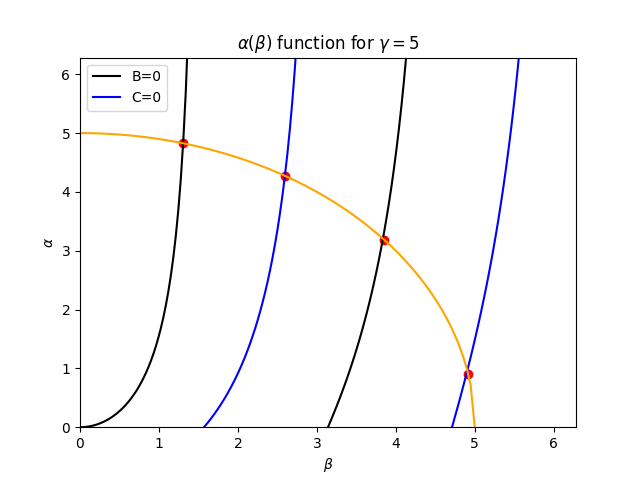
\includegraphics{images3/alpha_beta.png}
    \caption{$\alpha$ as a function of $\beta$ for $\gamma = 5$}
    \labfig{alpha_beta}
\end{figure}

This proves that the energy is quantized because only some values for $\alpha$ (that is a function of Energy) are possible.

And the solutions are:

Solution for C = 0
\begin{equation}
     \begin{split}
        & A = B sin(\beta)
        \\
        & B = B
        \\
        & C = 0
        \\
        & D = - B sin(\beta)
     \end{split}
\end{equation}

Solution for B = 0
\begin{equation}
     \begin{split}
        & A = C cos(\beta)
        \\
        & B = 0
        \\
        & C = C
        \\
        & D = C cos(\beta)
     \end{split}
\end{equation}



We still have one variable left to resolve, to do this we will need to use \ref{3.3}. We will resolve only for the case B = 0, the other one will turn the same.

\begin{equation}
    \label{3.29}
    \begin{split}
        & \int_{-\infty}^{\infty} \phi^2(x) dx = 
        \\
        & = C^2\left[ cos^2(\beta) \int_{-\infty}^{-a}e^{\frac{2\alpha}{a}x}dx + e^{-2\alpha}\int_{-a}^{a} cos^2(\frac{\beta}{a}x) dx + cos^2(\beta) \int_{a}^{\infty}e^{-\frac{2\alpha}{a}x}dx \right]=
        \\
        & =  C^2\left[ cos^2(\beta)\frac{a}{2\alpha} \left[e^{\frac{2\alpha}{a}x}\right]_{-\infty}^{-a} 
        + \frac{e^{-2\alpha}}{2} \left[\frac{a}{2\beta}sin(\frac{2\beta}{a}x)+x\right]_{-a}^{a} 
        - cos^2(\beta) \frac{a}{2\alpha} \left[e^{\frac{2\alpha}{a}x}\right]_{a}^{\infty} \right] =
        \\
        & C^2 a e^{-2\alpha}\left[\frac{cos^2(\beta)}{\beta\tan{(\beta)}}+\frac{sin(2\beta)}{2\beta}+1\right] =
        \\
        & = C^2ae^{-2\alpha}\left[\frac{1}{\alpha}+1\right] = 1
    \end{split}
\end{equation}

Now we need to resolve for C in the last step.

\begin{equation}
    \label{3.30}
    C^2 = \frac{\alpha e^{2\alpha}}{a(1+\alpha)}
\end{equation}

If C=0 then, $B^2$ is equal to the expression above. 

Now we can solve for everything in the problem for a given gamma.


\section{Examples}

We will plot some of the solutions for different gamma and for the largest gamma we will try to approach and explain a classical behaviour.

\textbf{First example: } In this case we will took gamma = 10, and plot two of the solutions, one for B=0 and the other one for C=0.

\begin{figure}[H]
    \centering
    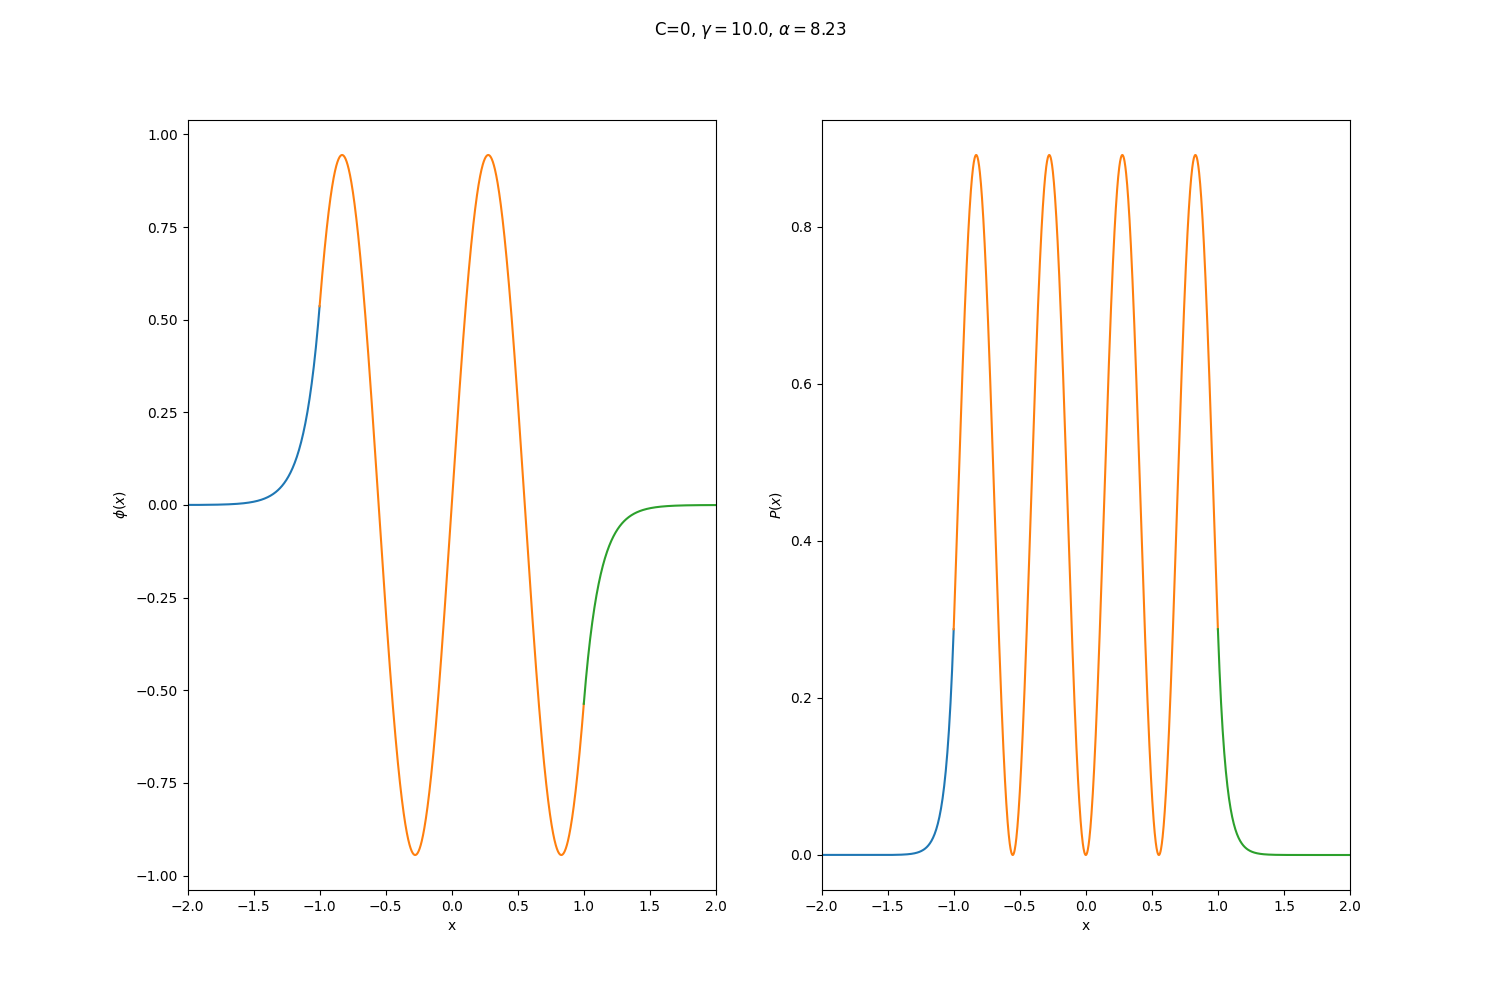
\includegraphics{images3/phi_gamma=10.0_alpha=8.23.png}
    \caption{$\phi(x)$ and P(x) functions for gamma = 10}
    \label{gamma1=10}
\end{figure}

\begin{figure}[H]
    \centering
    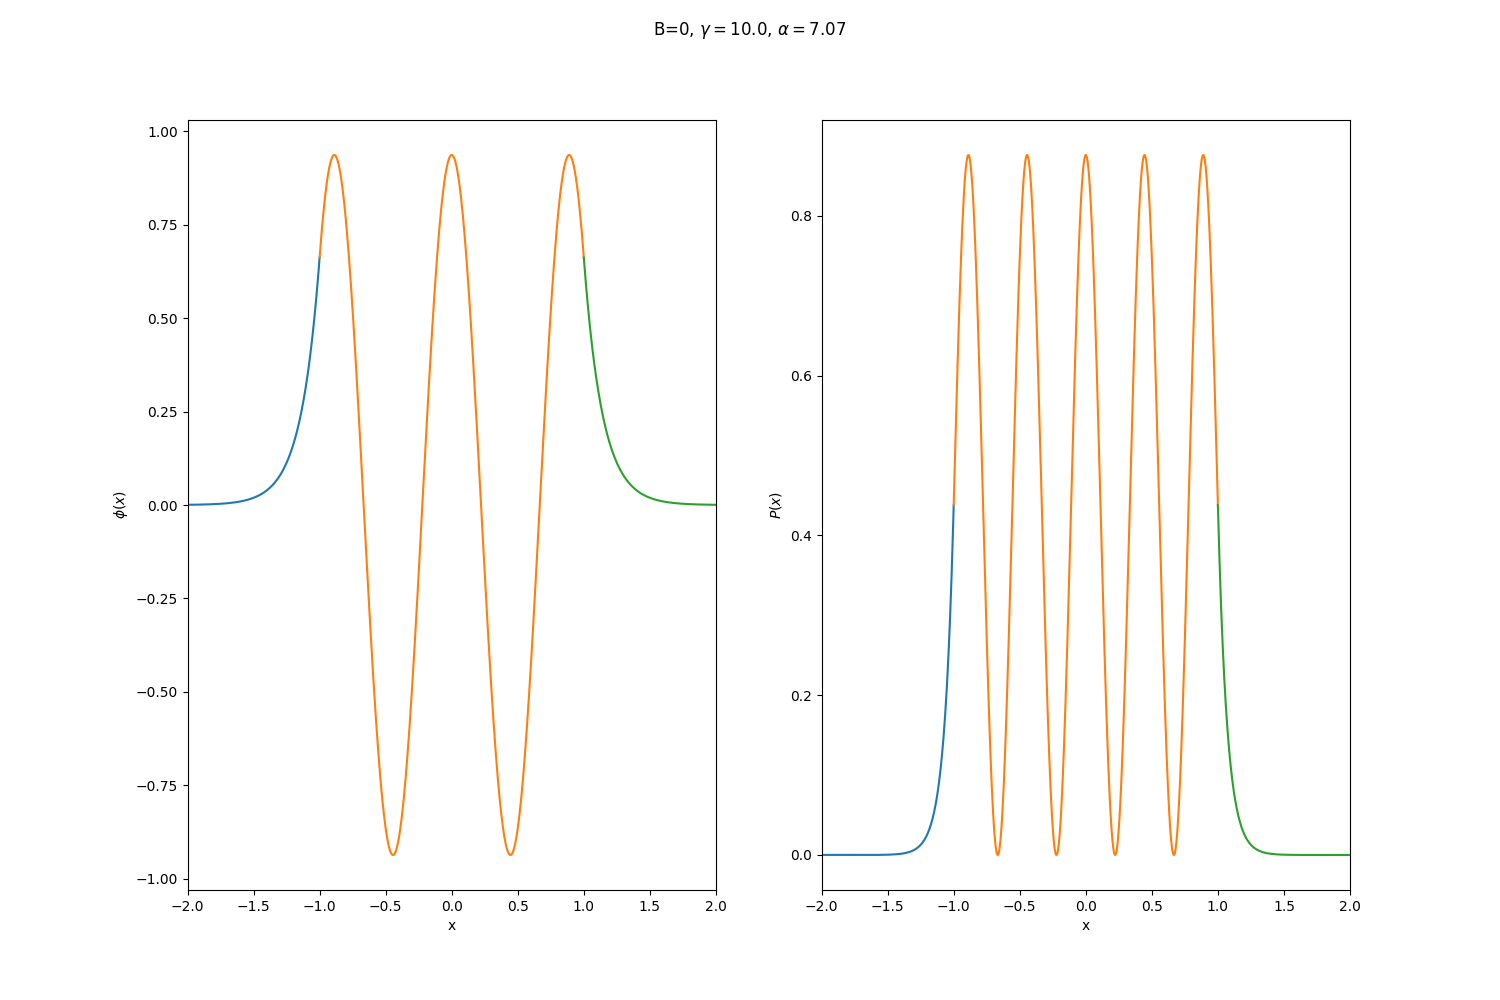
\includegraphics{images3/phi_gamma=10.0_alpha=7.07.png}
    \caption{$\phi(x)$ and P(x) functions for gamma = 10}
    \label{gamma2=10}
\end{figure}

Now we will try to achieve a similar behaviour to the well-known particle approach, where all the probability is inside the square root potential and all of it is equally likely to have the particle. We can achieve this finding the P(x) function for a bigger gamma and a small alpha.

\begin{figure}[H]
    \centering
    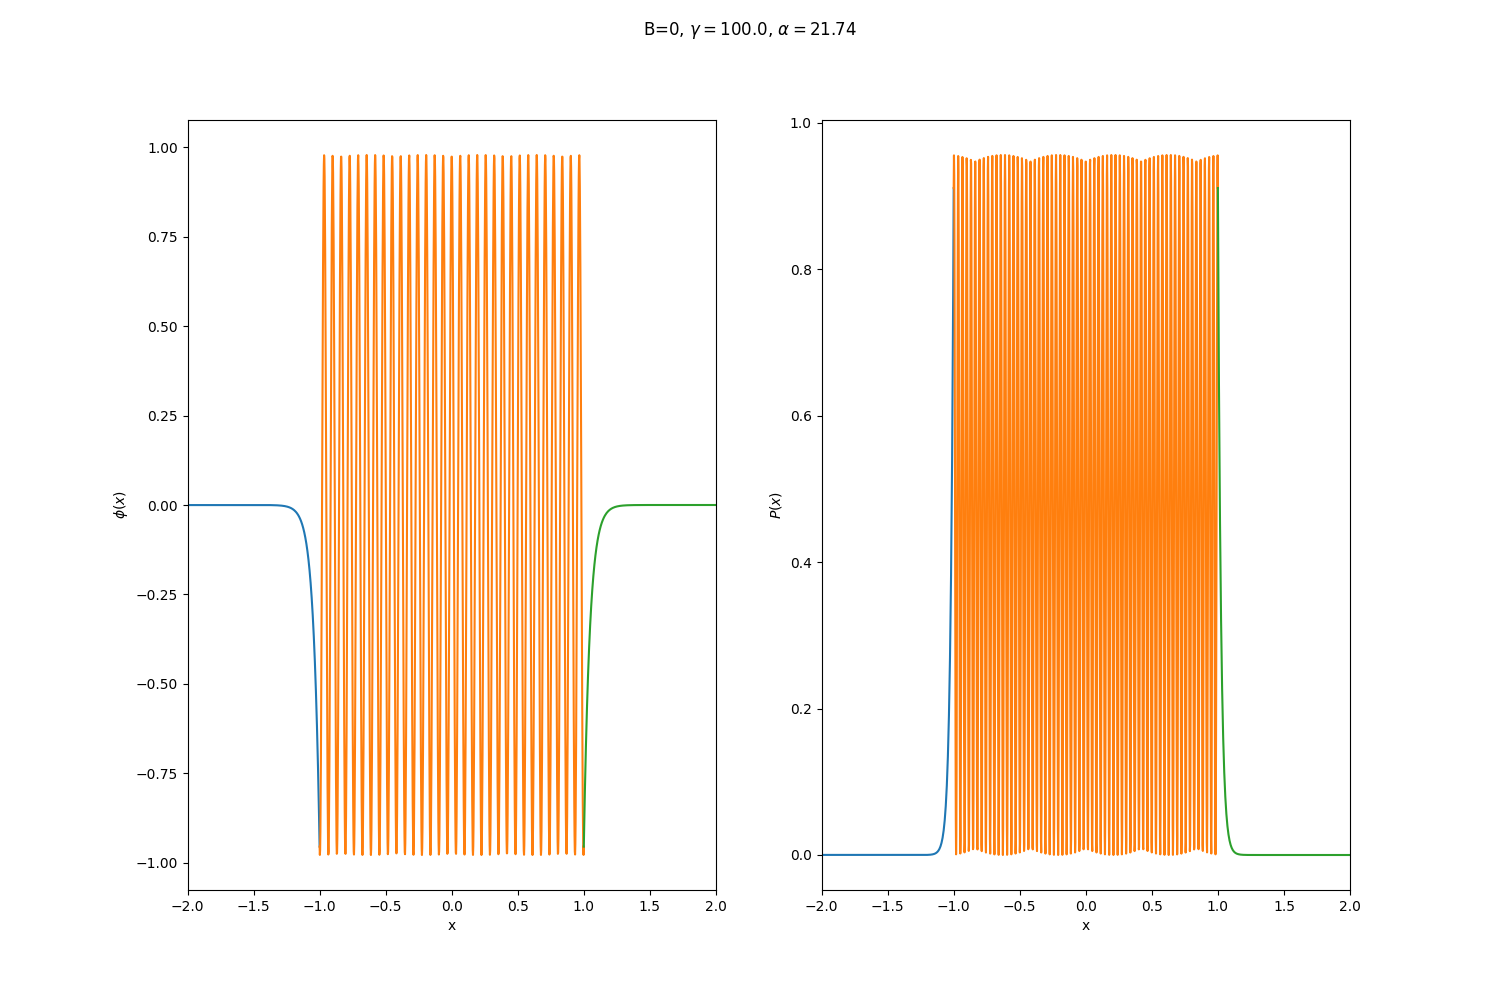
\includegraphics{images3/phi_gamma=100.0_alpha=21.74.png}
    \caption{$\phi(x)$ and P(x) functions for gamma = 100}
    \labfig{gamma=100}
\end{figure}

In \reffig{gamma=100} we can see that we get what we expect for a particle behaviour but we still have that quantum behaviour because the integral outside of the square potential is not zero as it should be in the particle behaviour.


% \setchapterimage[7.5cm]{seaside}
% \setchapterpreamble[u]{\margintoc}
% %\chapter[Figures and Tables]{Figures and Tables\footnotemark[0]}
% \chapter{Figures and Tables}

% \footnotetext{The credits for the image above the chapter title go to:
% 	Bushra Feroz, CC~BY-SA~4.0, \url{https://commons.wikimedia.org/w/index.php?curid=68724647}}

% \section{Normal Figures and Tables}

% Figures and tables can be inserted just like in any standard 
% \LaTeX\xspace document. The \Package{graphicx} package is already loaded 
% and configured in such a way that the figure width is equal to the 
% textwidth and the height is adjusted in order to maintain the original 
% aspect ratio. As you may have imagined, the captions will be 
% positioned\ldots well, in the margins. This is achieved with the help of 
% the \Package{floatrow} package.

% Here is a picture of Mona Lisa (\reffig{normalmonalisa}), as an example. 
% The captions are formatted as the margin- and the side-notes; If you 
% want to change something about captions you can use the command 
% \Command{captsetup} from the \Package{caption} package. Remember that if 
% you want to reference a figure, the label must come \emph{after} the 
% caption!

% \begin{figure}[hb]
% 	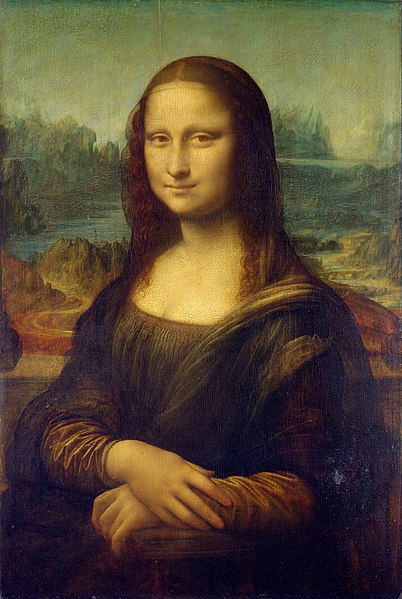
\includegraphics[width=0.45\textwidth]{monalisa}
% 	\caption[Mona Lisa, again]{It's Mona Lisa again. \blindtext}
% 	\labfig{normalmonalisa}
% \end{figure}

% While the format of the caption is managed by \Package{caption}, its 
% position is handled by the \Package{floatrow} package. Achieving this 
% result has been quite hard, but now I am pretty satisfied. In two-side 
% mode, the captions are printed in the correct margin.

% Tables can be inserted just as easily as figures, as exemplified by the 
% following code:

% \begin{lstlisting}[caption={Caption of a listing.}]
% \begin{table}
% \begin{tabular}{ c c c c }
% 	\toprule
% 	col1 & col2 & col3 & col 4 \\
% 	\midrule
% 	\multirow{3}{4em}{Multiple row} & cell2 & cell3 & cell4\\ &
% 	cell5 & cell6 & cell7 \\ &
% 	cell8 & cell9 & cell10 \\
% 	\multirow{3}{4em}{Multiple row} & cell2 & cell3 & cell4 \\ &
% 	cell5 & cell6 & cell7 \\ &
% 	cell8 & cell9 & cell10 \\
% 	\bottomrule
% \end{tabular}
% \end{table}
% \end{lstlisting}

% which results in the useless \vreftab{useless}.

% \begin{table}[ht]
% \caption[A useless table]{A useless table.}
% \labtab{useless}
% \begin{tabular}{ c c c c }
% 	\toprule
% 	col1 & col2 & col3 & col 4 \\
% 	\midrule
% 	\multirow{3}{4em}{Multiple row} & cell2 & cell3 & cell4\\ &
% 	cell5 & cell6 & cell7 \\ &
% 	cell8 & cell9 & cell10 \\
% 	\multirow{3}{4em}{Multiple row} & cell2 & cell3 & cell4 \\ &
% 	cell5 & cell6 & cell7 \\ &
% 	cell8 & cell9 & cell10 \\
% 	\bottomrule
% \end{tabular}
% \end{table}

% I don't have much else to say, so I will just insert some blind text. 
% \blindtext

% \section{Margin Figures and Tables}

% Marginfigures can be inserted with the environment 
% \Environment{marginfigure}. In this case, the whole picture is confined 
% to the margin and the caption is below it. \reffig{marginmonalisa} is 
% obtained with something like this:

% \begin{lstlisting}[caption={Another caption.}]
% \begin{marginfigure}
% 	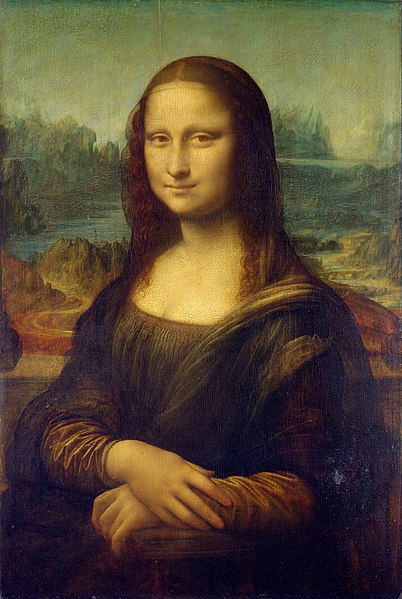
\includegraphics{monalisa}
% 	\caption[The Mona Lisa]{The Mona Lisa.}
% 	\labfig{marginmonalisa}
% \end{marginfigure}
% \end{lstlisting}

% There is also the \Environment{margintable} environment, of which 
% \reftab{anotheruseless} is an example. Notice how you can place the 
% caption above the table by just placing the \Command{caption} command 
% before beginning the \Environment{tabular} environment. Usually, figure 
% captions are below, while table captions are above. This rule is also 
% respected for normal figures and tables: the captions are always on the 
% side, but for figure they are aligned to the bottom, while for tables to 
% the top.

% \begin{margintable}
% \caption[Another useless table]{Another useless table.}
% \labtab{anotheruseless}
% \raggedright
% \begin{tabular}{ c c c c }
% 	\hline
% 	col1 & col2 & col3 \\
% 	\hline
% 	\multirow{3}{4em}{Multiple row} & cell2 & cell3 \\ & cell5 & cell6 
% 	\\ & cell8 & cell9 \\ \hline
% \end{tabular}
% \end{margintable}

% Marginfigures and tables can be positioned with an optional offset 
% command, like so:

% \begin{lstlisting}
% \begin{marginfigure}[offset]
% 	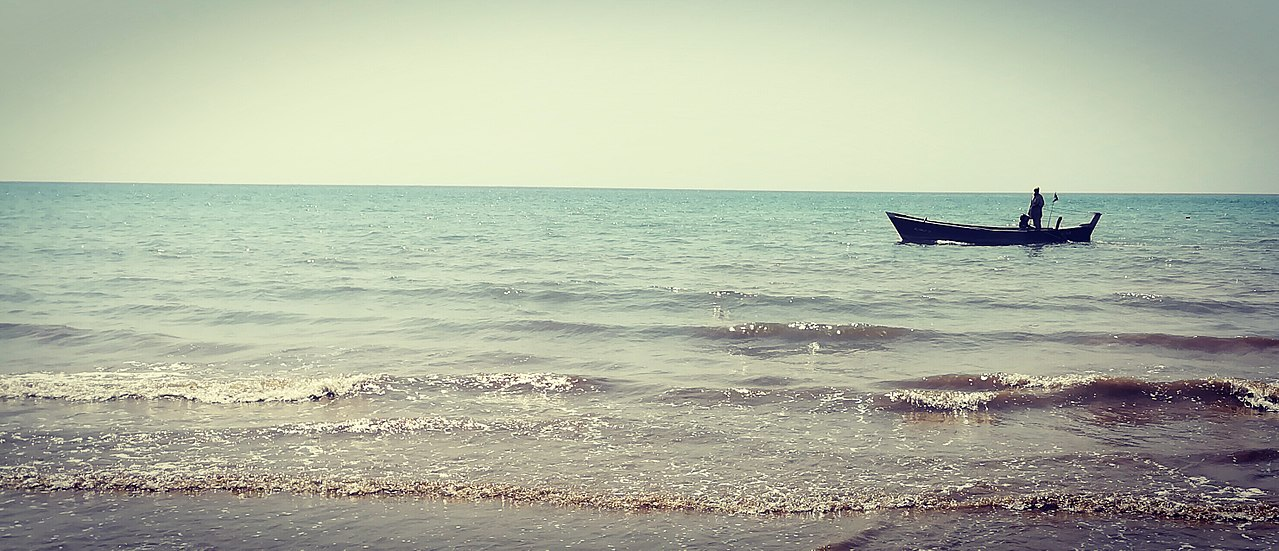
\includegraphics{seaside}
% \end{marginfigure}
% \end{lstlisting}

% Offset ca be either a measure or a multiple of \Command{baselineskip}, 
% much like with \Command{sidenote}, \Command{marginnote} and 
% \Command{margintoc}.\todo{Improve this part.} If you are wondering how I 
% inserted this orange bubble, have a look at the \Package{todo} package.

% \section{Wide Figures and Tables}

% With the environments \Environment{figure*} and \Environment{table*} you 
% can insert figures which span the whole page width. For example, here 
% are a wide figure and a wide table.

% \begin{figure*}[h!]
% 	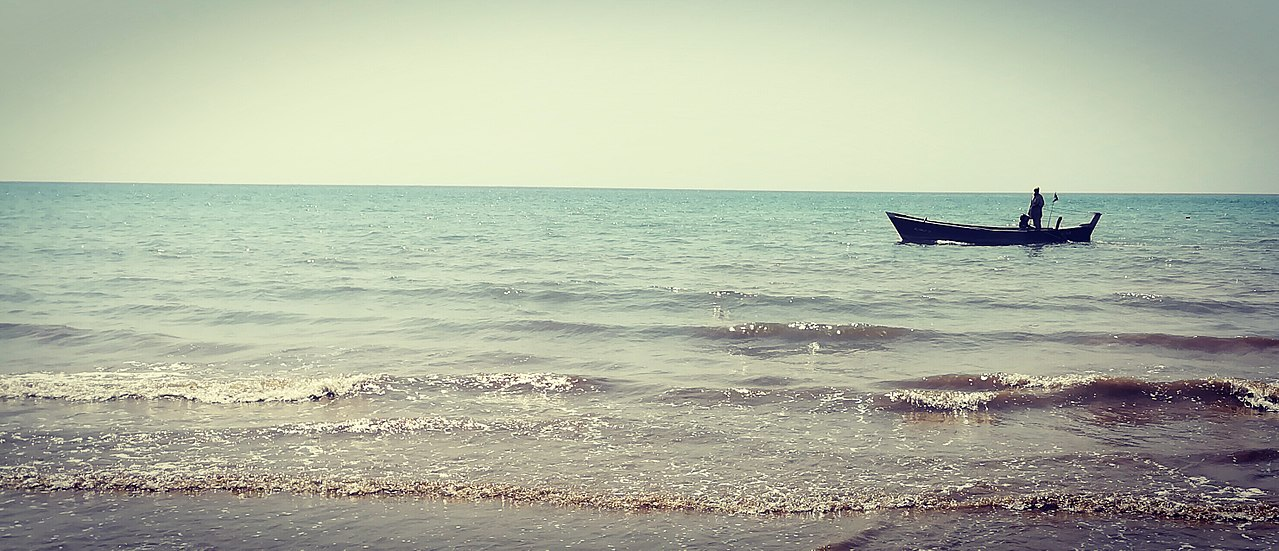
\includegraphics{seaside}
% 	\caption[A wide seaside]{A wide seaside, and a wide caption.
% 		Credits: By Bushra Feroz, CC BY-SA 4.0, \url{https://commons.wikimedia.org/w/index.php?curid=68724647}}
% \end{figure*}

% \begin{table*}[h!]
%     \caption{A wide table with invented data about three people living in the UK. Note that wide figures and tables are centered and their caption also extends into the margin.}
%     \begin{tabular}{p{2.0cm} p{2.0cm} p{2.0cm} p{2.0cm} p{2.0cm} p{2.0cm} p{1.5cm}}
%         \toprule
%         Name    & Surname   & Job       & Salary           & Age   & Height    & Country \\
%         \midrule
%         Alice   & Red       & Writer    & 4.000 \pounds    & 34    & 167 cm     & England \\
%         Bob     & White     & Bartender & 2.000 \pounds    & 24    & 180 cm     & Scotland \\
%         Drake   & Green     & Scientist & 4.000 \pounds    & 26    & 175 cm     & Wales \\
%         \bottomrule
%     \end{tabular}
% \end{table*}

% It is the user's responsibility to adjust the width of the table, if 
% necessary, until it is aesthetically pleasing. The previous table was 
% obtained with the following code:

% \begin{lstlisting}[caption=How to typeset a wide table]
% \begin{table*}[h!]
%     \caption{A wide table with invented data about three people living in the UK. Note that wide figures and tables are centered and their caption also extends into the margin.}
%     \begin{tabular}{p{2.0cm} p{2.0cm} p{2.0cm} p{2.0cm} p{2.0cm} p{2.0cm} p{1.5cm}}
%         \toprule
%         Name    & Surname   & Job       & Salary           & Age   & Height    & Country \\
%         \midrule
%         Alice   & Red       & Writer    & 4.000 \pounds    & 34    & 167 cm     & England \\
%         Bob     & White     & Bartender & 2.000 \pounds    & 24    & 180 cm     & Scotland \\
%         Drake   & Green     & Scientist & 4.000 \pounds    & 26    & 175 cm     & Wales \\
%         \bottomrule
%     \end{tabular}
% \end{table*}
% \end{lstlisting}

% The \Package{floatrow} package provides the \enquote{H} specifier to 
% instruct \LaTeX to position the figure (or table) in precisely the same 
% position it occupies in the source code. However, this specifier does 
% not work with wide figures or tables: you should use \enquote{h!} 
% instead, like so: \lstinline|\begin{figure*}[h!]|.

% You may have noticed the full width image at the very beginning of this
% chapter: that, however, is set up in an entirely different way, which
% you'll read about in \vrefch{layout}.

% \Class{kaobook} also supports paginated tables (have a look at the 
% \Package{longtable} package). The 
% \Environment{longtable}\sidenote{Interestingly, \Environment{longtable}s 
% may require up to four rounds of compilation before they are typeset 
% correctly.} environment behaves a bit differently from 
% \Environment{table}, in that \Environment{longtable} encompasses both 
% \Environment{table} and \Environment{tabular}, so that you can write, 
% \eg,

% \begin{lstlisting}[caption=Example of a longtable]
% \begin{longtable}{|l c c|}
%     \hline
%     One & Two & Three \\
%     Left & Center & Center \\
%     \hline
%     \caption{Caption of the longtable.}
% \end{longtable}
% \end{lstlisting}

% to obtain the following table:
% \begin{longtable}{|l c c|}
%     \hline
%     One & Two & Three \\
%     Left & Center & Center \\
%     \hline
%     \caption{Caption of the longtable.}
% \end{longtable}

% The caption of a \Environment{longtable} is always positioned below the 
% table, and it has the same width as the text (it doesn't extend into the 
% margin). However, sometimes you may need a \Environment{longtable} that 
% is so wide that it trespass into the margins; in those cases, you may 
% want to also increase the width of the caption. To do so, you'll have to 
% write two additional commands, one before and one after the 
% \Environment{longtable}:

% \begin{lstlisting}[caption=Increasing the width of the caption of a \Environment{longtable}.]
% \floatsetup[longtable]{margins=centering,LTcapwidth=table} % Add this line before the longtable to increase the caption width
% \begin{longtable}{lp{8cm}p{5cm}p{2cm}}
% ...
% \end{longtable}
% \floatsetup[longtable]{margins=raggedright,LTcapwidth=\textwidth} % Add this line after the longtable to revert the previous change
% \end{lstlisting}

% Having seen figures and tables, it is now time to tackle 
% hyperreferences.
